\documentclass{beamer}
\usepackage{pgfpages}
\usepackage[backend=bibtex]{biblatex}
\usepackage{multicol}
\usepackage{multimedia}
\usepackage[absolute,overlay]{textpos}
\usepackage{parskip}
\usepackage{hyperref}
\usepackage{lmodern}
\usepackage{bbding}
\usepackage[absolute,overlay]{textpos}
\hypersetup{colorlinks=true, urlcolor=blue}
\setlength{\parskip}{\smallskipamount} 
%\usepackage[texcoord,grid,gridunit=mm,gridcolor=red!10,subgridcolor=green!10]{eso-pic} %DELETE when done with grid
\setbeameroption{hide notes} % Only slides
%\setbeameroption{show only notes} % Only notes
%\setbeameroption{show notes on second screen=right} % Both
%\bibliography{../../papers/references.bib}
\setbeamerfont{footnote}{size=\tiny}
%\AtEveryCitekey{\clearfield{title}}

%
% Choose how your presentation looks.
%
% For more themes, color themes and font themes, see:
% http://deic.uab.es/~iblanes/beamer_gallery/index_by_theme.html
%
\mode<presentation>
{
  \usetheme{Warsaw}      % or try Darmstadt, Madrid, Warsaw, ...
  \usecolortheme{default} % or try albatross, beaver, crane, ...
  \usefonttheme{default}  % or try serif, structurebold, ...
  \setbeamertemplate{navigation symbols}{}
  \setbeamertemplate{caption}[numbered]
} 

\usepackage[english]{babel}
%\usepackage[utf8x]{inputenc} %Doesn't play well with biblatex
\usepackage{amssymb}
\usepackage{bm}
\usepackage{color}
\usepackage{graphicx}
\setbeamercovered{invisible}
\setbeamercovered{%
  again covered={\opaqueness<1->{25}}}

\newcommand{\red}[1]{{\color{red}{#1}}}
\newcommand{\checkH}[2]{\begin{textblock*}{1cm}(#1,#2){\Huge \red{\Checkmark}}\end{textblock*}}

\title[{\color{white}{Chapters 1.1-3}}]{Physics 121: \\ Intro; Motion Diagrams; x vs. t}
\author{Cody Petrie}
\institute{Mesa Community College}
\date{}

\begin{document}

%\setbeamertemplate{frametitle}[default][center]
\begin{frame}
   \titlepage
\end{frame}

% Uncomment these lines for an automatically generated outline.
%\begin{frame}{Outline}
%  \tableofcontents
%\end{frame}

% Commands to include a figure:
%\begin{figure}
%\includegraphics[width=\textwidth]{your-figure's-file-name}
%\caption{\label{fig:your-figure}Caption goes here.}
%\end{figure}

\iffalse
\begin{frame}{Introduction}
\begin{center}
   \color{blue}{{\huge Two Truths and a Lie}}
   \\ I'll give you a minute to think while I introduce myself
\end{center}
\end{frame}

\begin{frame}{Family}
   \begin{itemize}
      \item Undergraduate degree from BYU in Physics with a minor in Astronomy. Now I'm in physics PhD program at ASU where I do computational nuclear physics.      \item At BYU I met my beautiful wife and we got married. 
      \item We have three kids, Ammon (4.9), Cooper (3) and Olivia (0.5)
   \end{itemize}
   \begin{center}
      \includegraphics[width=0.5\textwidth, angle=180, origin=c]{../figures/family1.jpg}
      ~ ~
      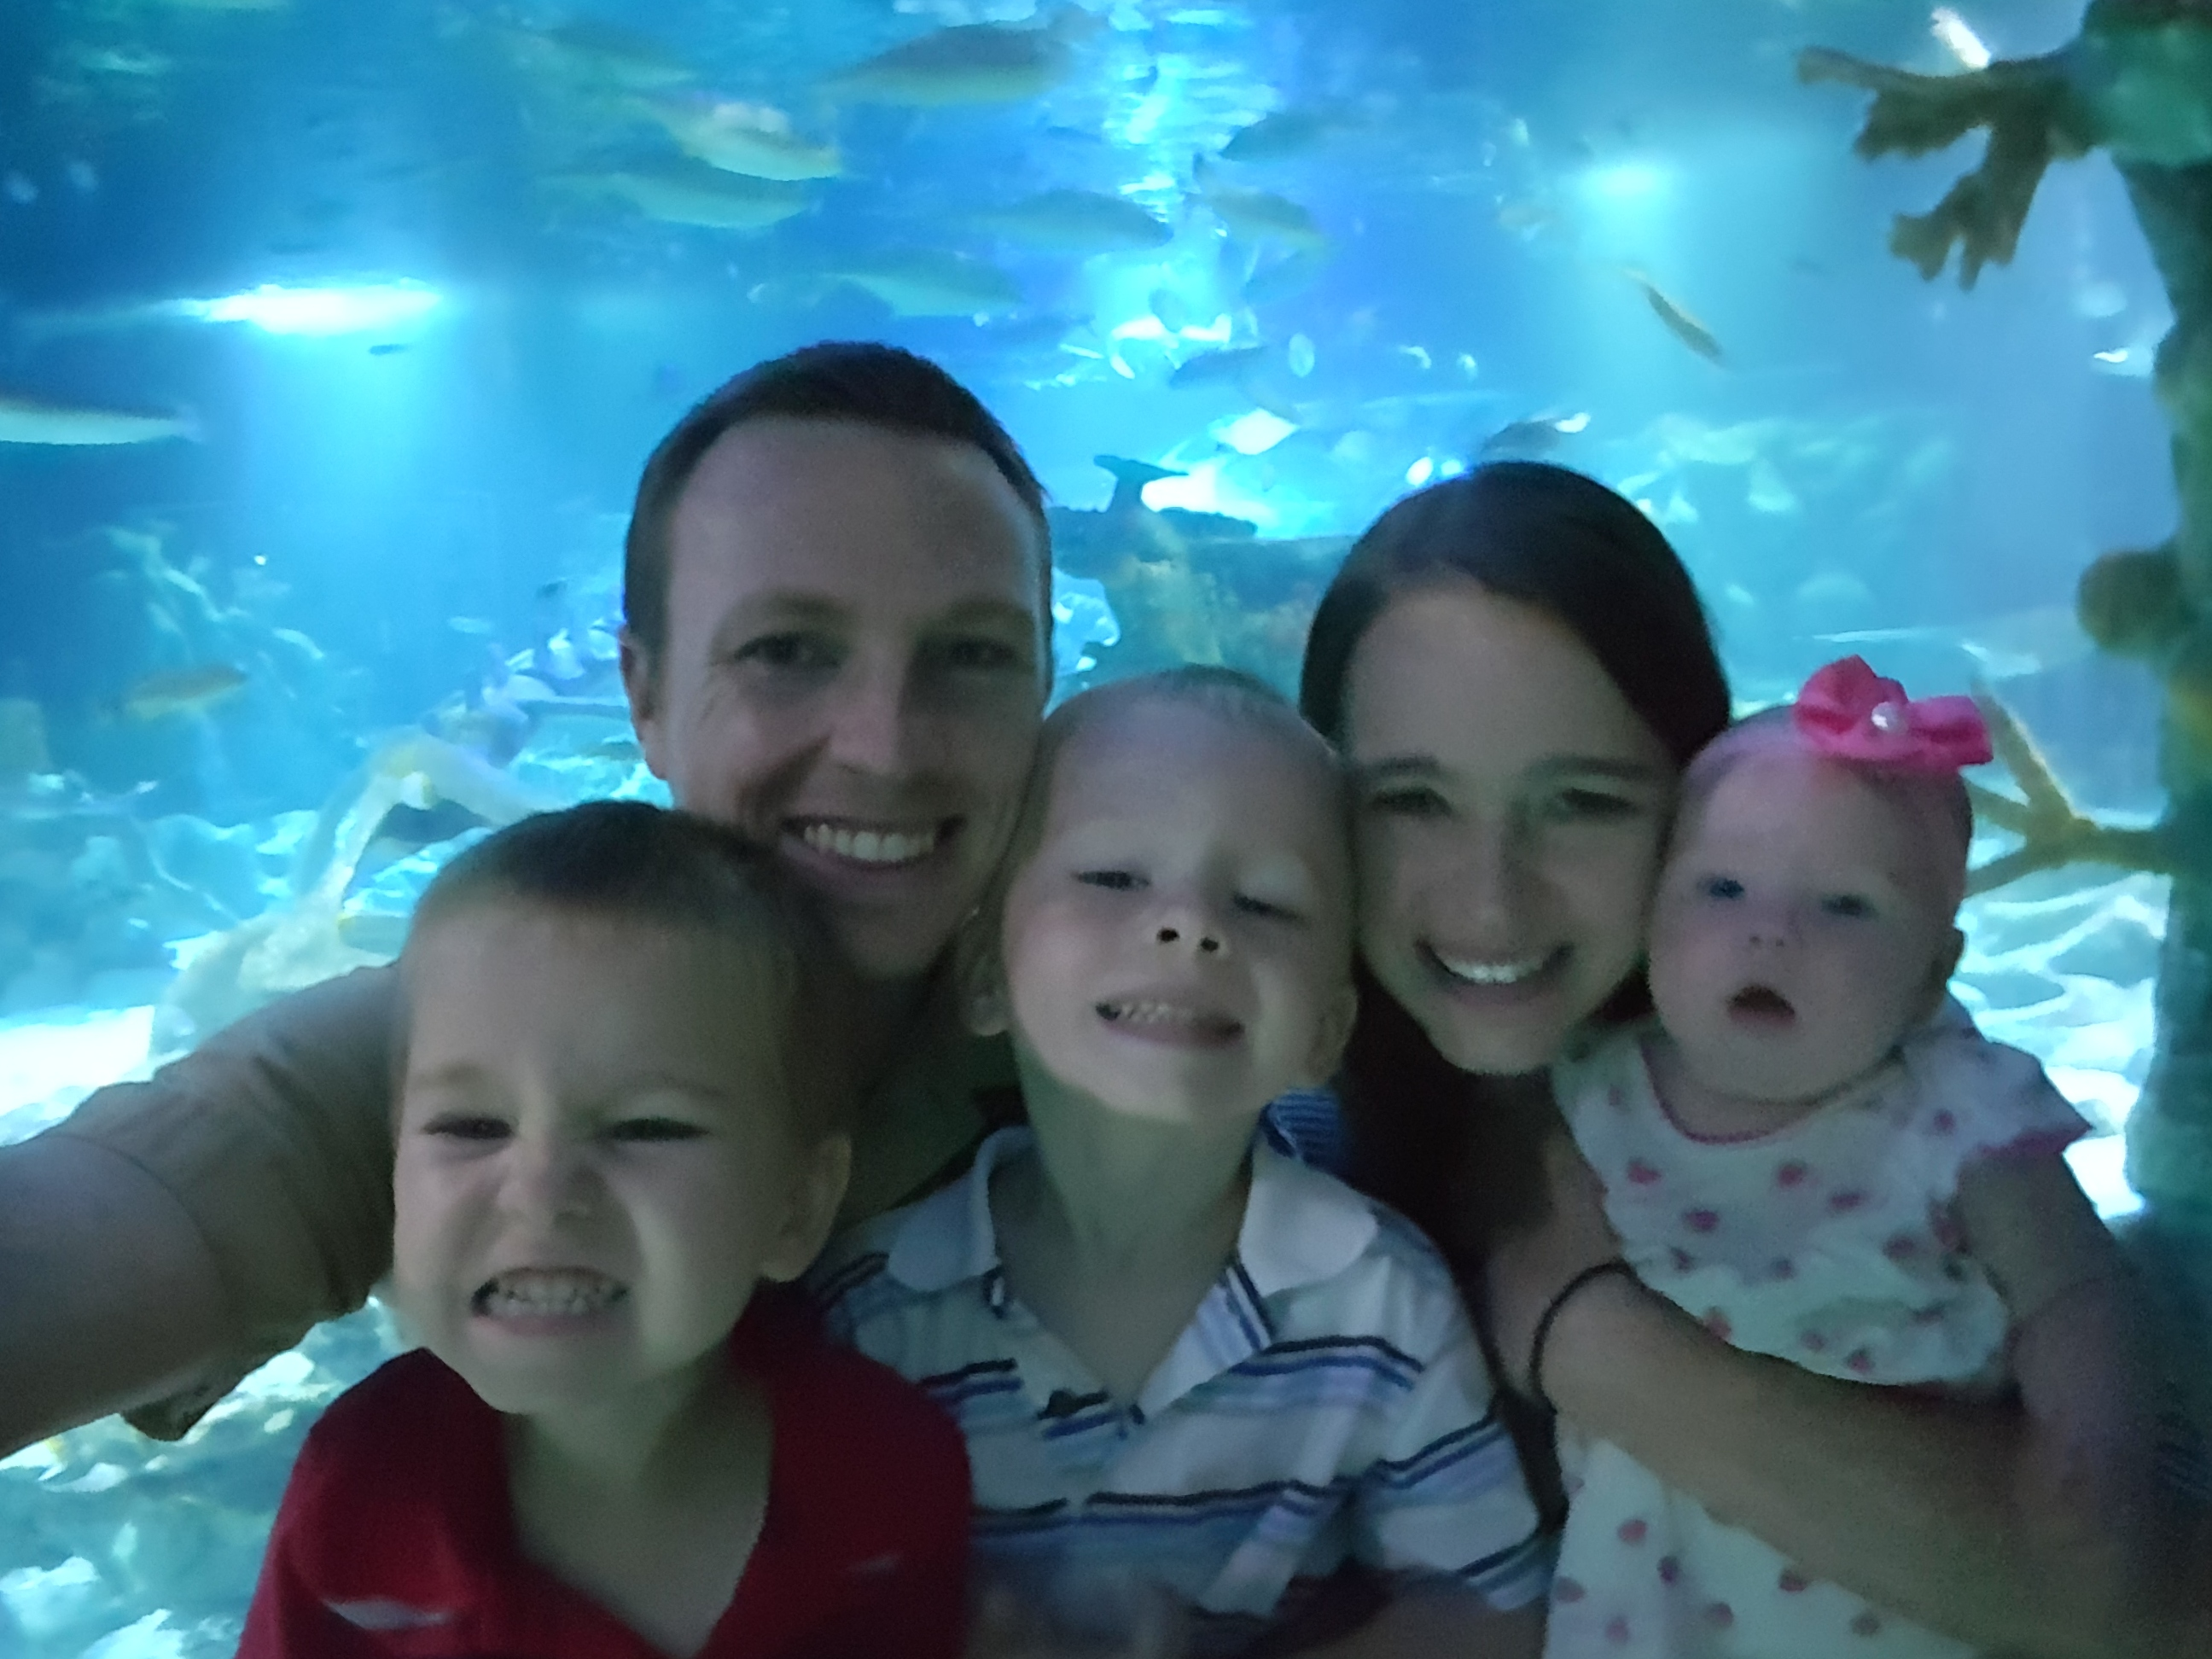
\includegraphics[width=0.5\textwidth]{../figures/family2.jpg}
   \end{center}
\end{frame}

\begin{frame}{Hobbies}
   \begin{textblock*}{\textwidth}(0.3cm,0.8cm) % {block width} (coords)
      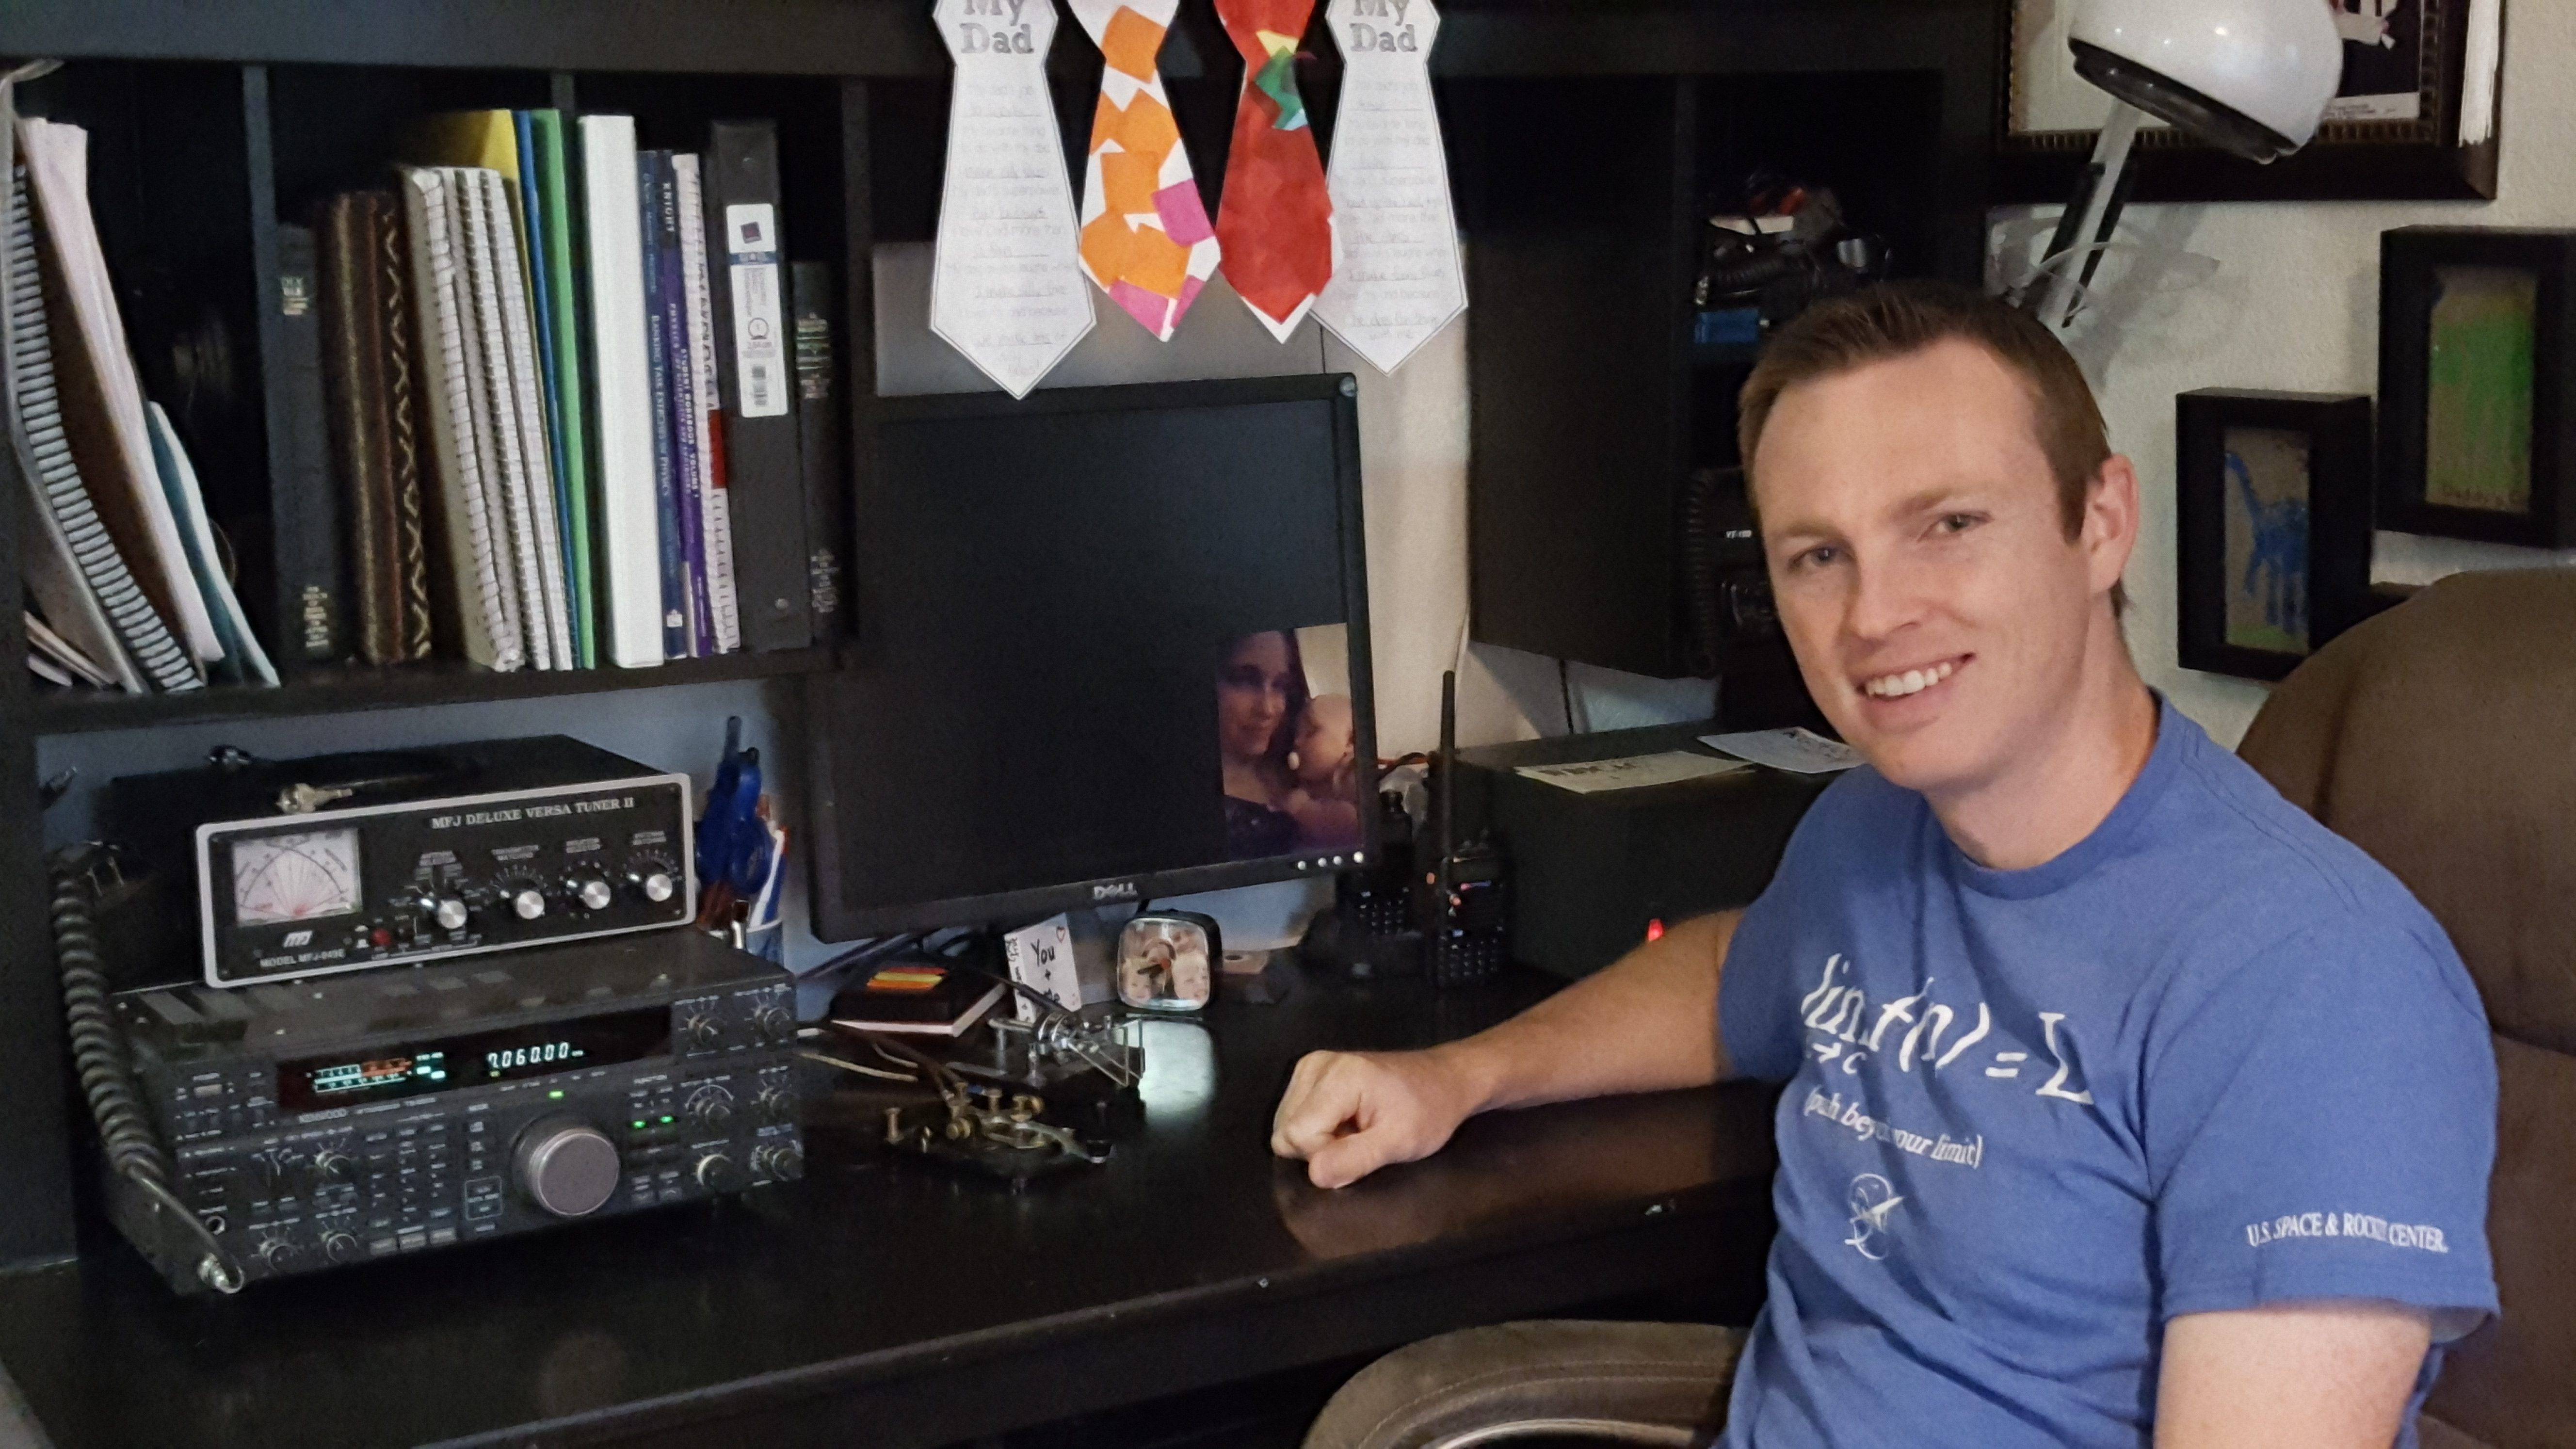
\includegraphics[width=4.0cm]{../figures/radio.jpg}
   \end{textblock*}
   \begin{textblock*}{\textwidth}(4.5cm,0.8cm) % {block width} (coords)
      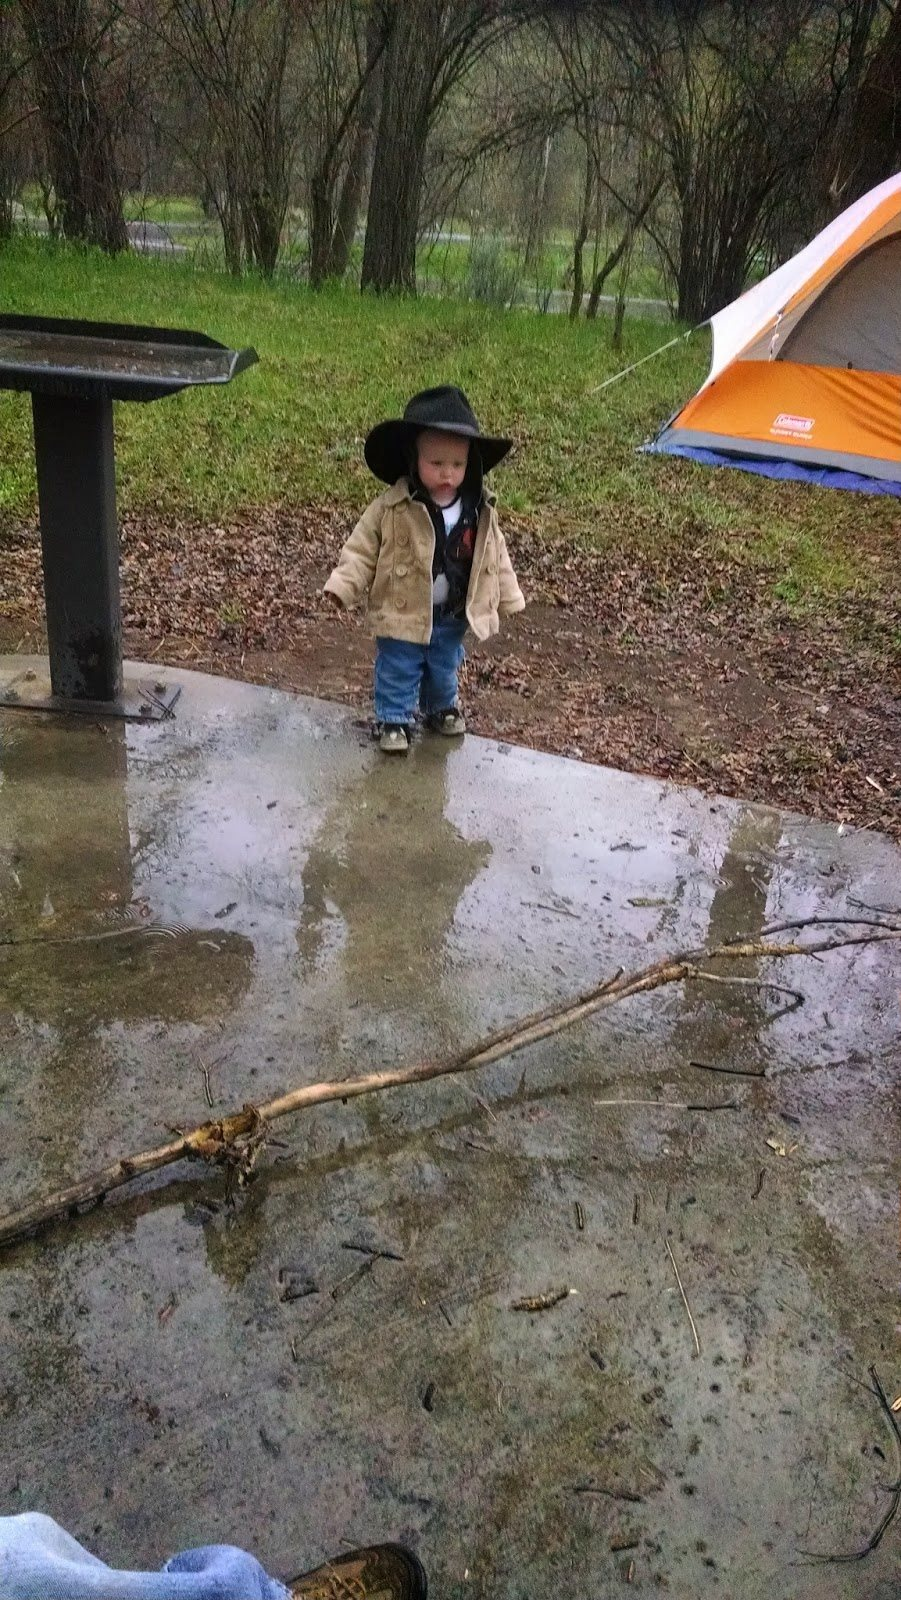
\includegraphics[width=3.5cm]{../figures/camping.jpg}
   \end{textblock*}
   \begin{textblock*}{\textwidth}(0.3cm,3.3cm) % {block width} (coords)
      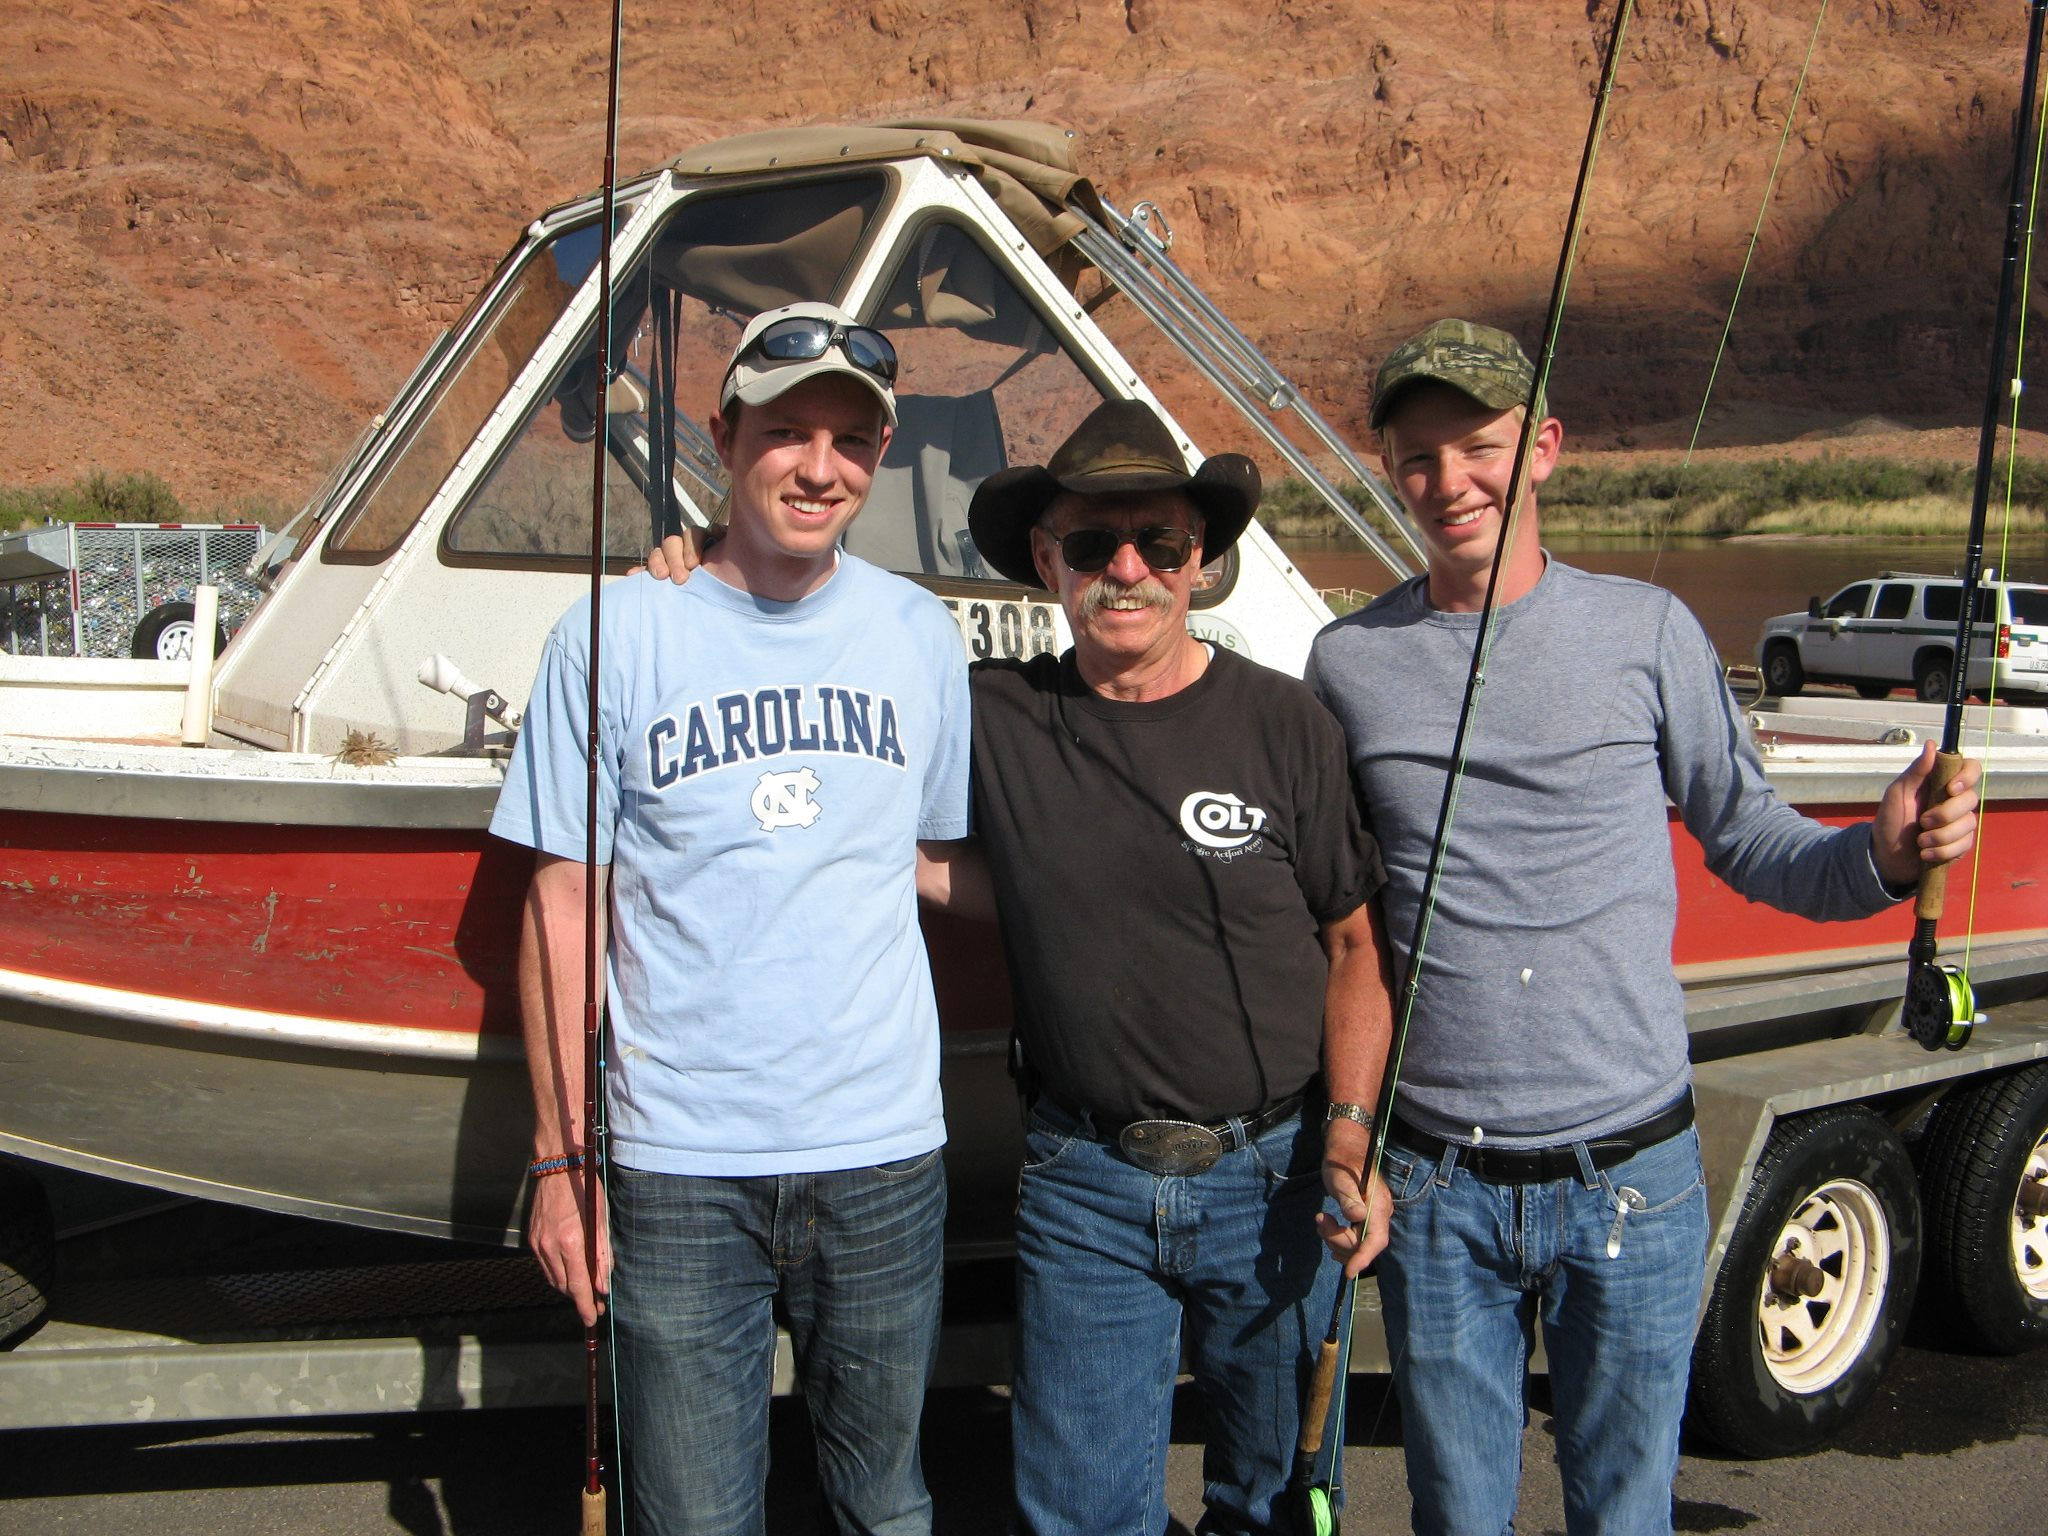
\includegraphics[width=3.5cm]{../figures/fishing.jpg}
   \end{textblock*}
   \begin{textblock*}{\textwidth}(8.5cm,0.8cm) % {block width} (coords)
      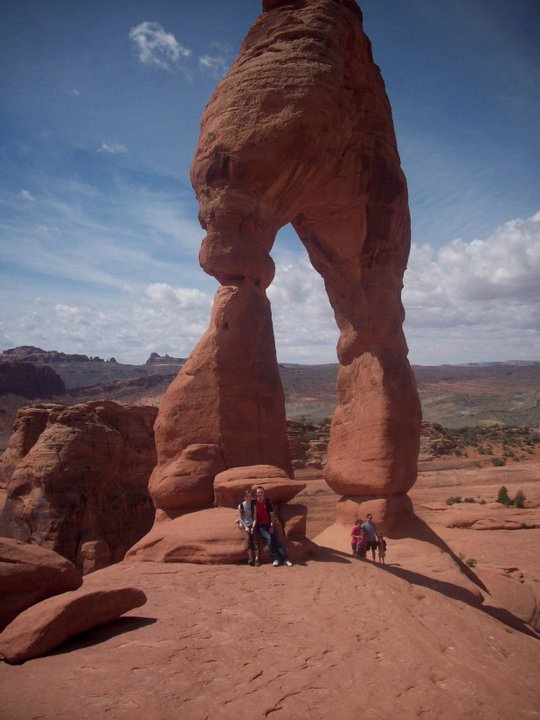
\includegraphics[width=3.5cm]{../figures/hiking.jpg}
   \end{textblock*}
   \begin{textblock*}{\textwidth}(0.3cm,6.3cm) % {block width} (coords)
      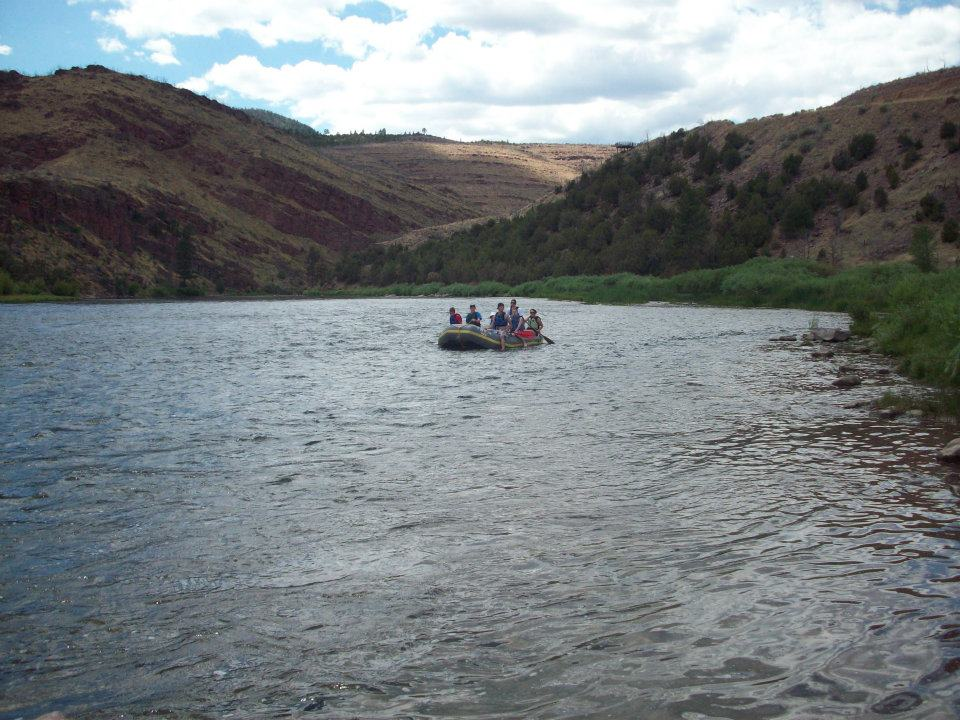
\includegraphics[width=3.5cm]{../figures/rafting.jpg}
   \end{textblock*}
   \begin{textblock*}{\textwidth}(8.5cm,6.3cm) % {block width} (coords)
      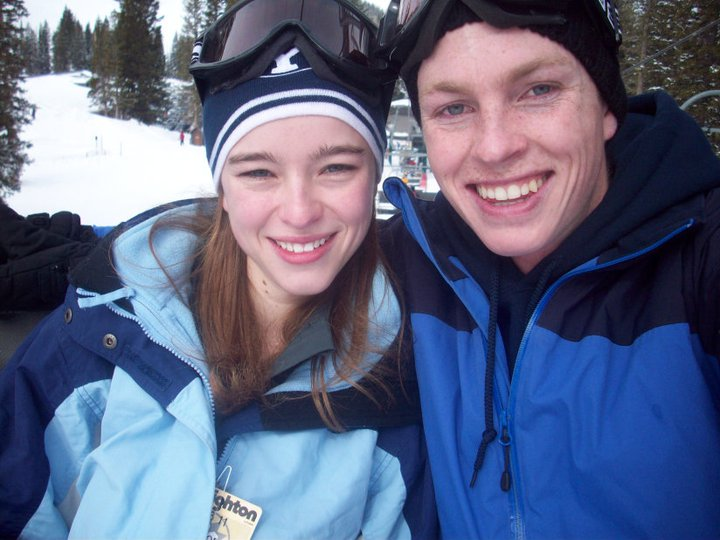
\includegraphics[width=3.5cm]{../figures/skiing.jpg}
   \end{textblock*}
   \begin{textblock*}{\textwidth}(4.4cm,6.1cm) % {block width} (coords)
      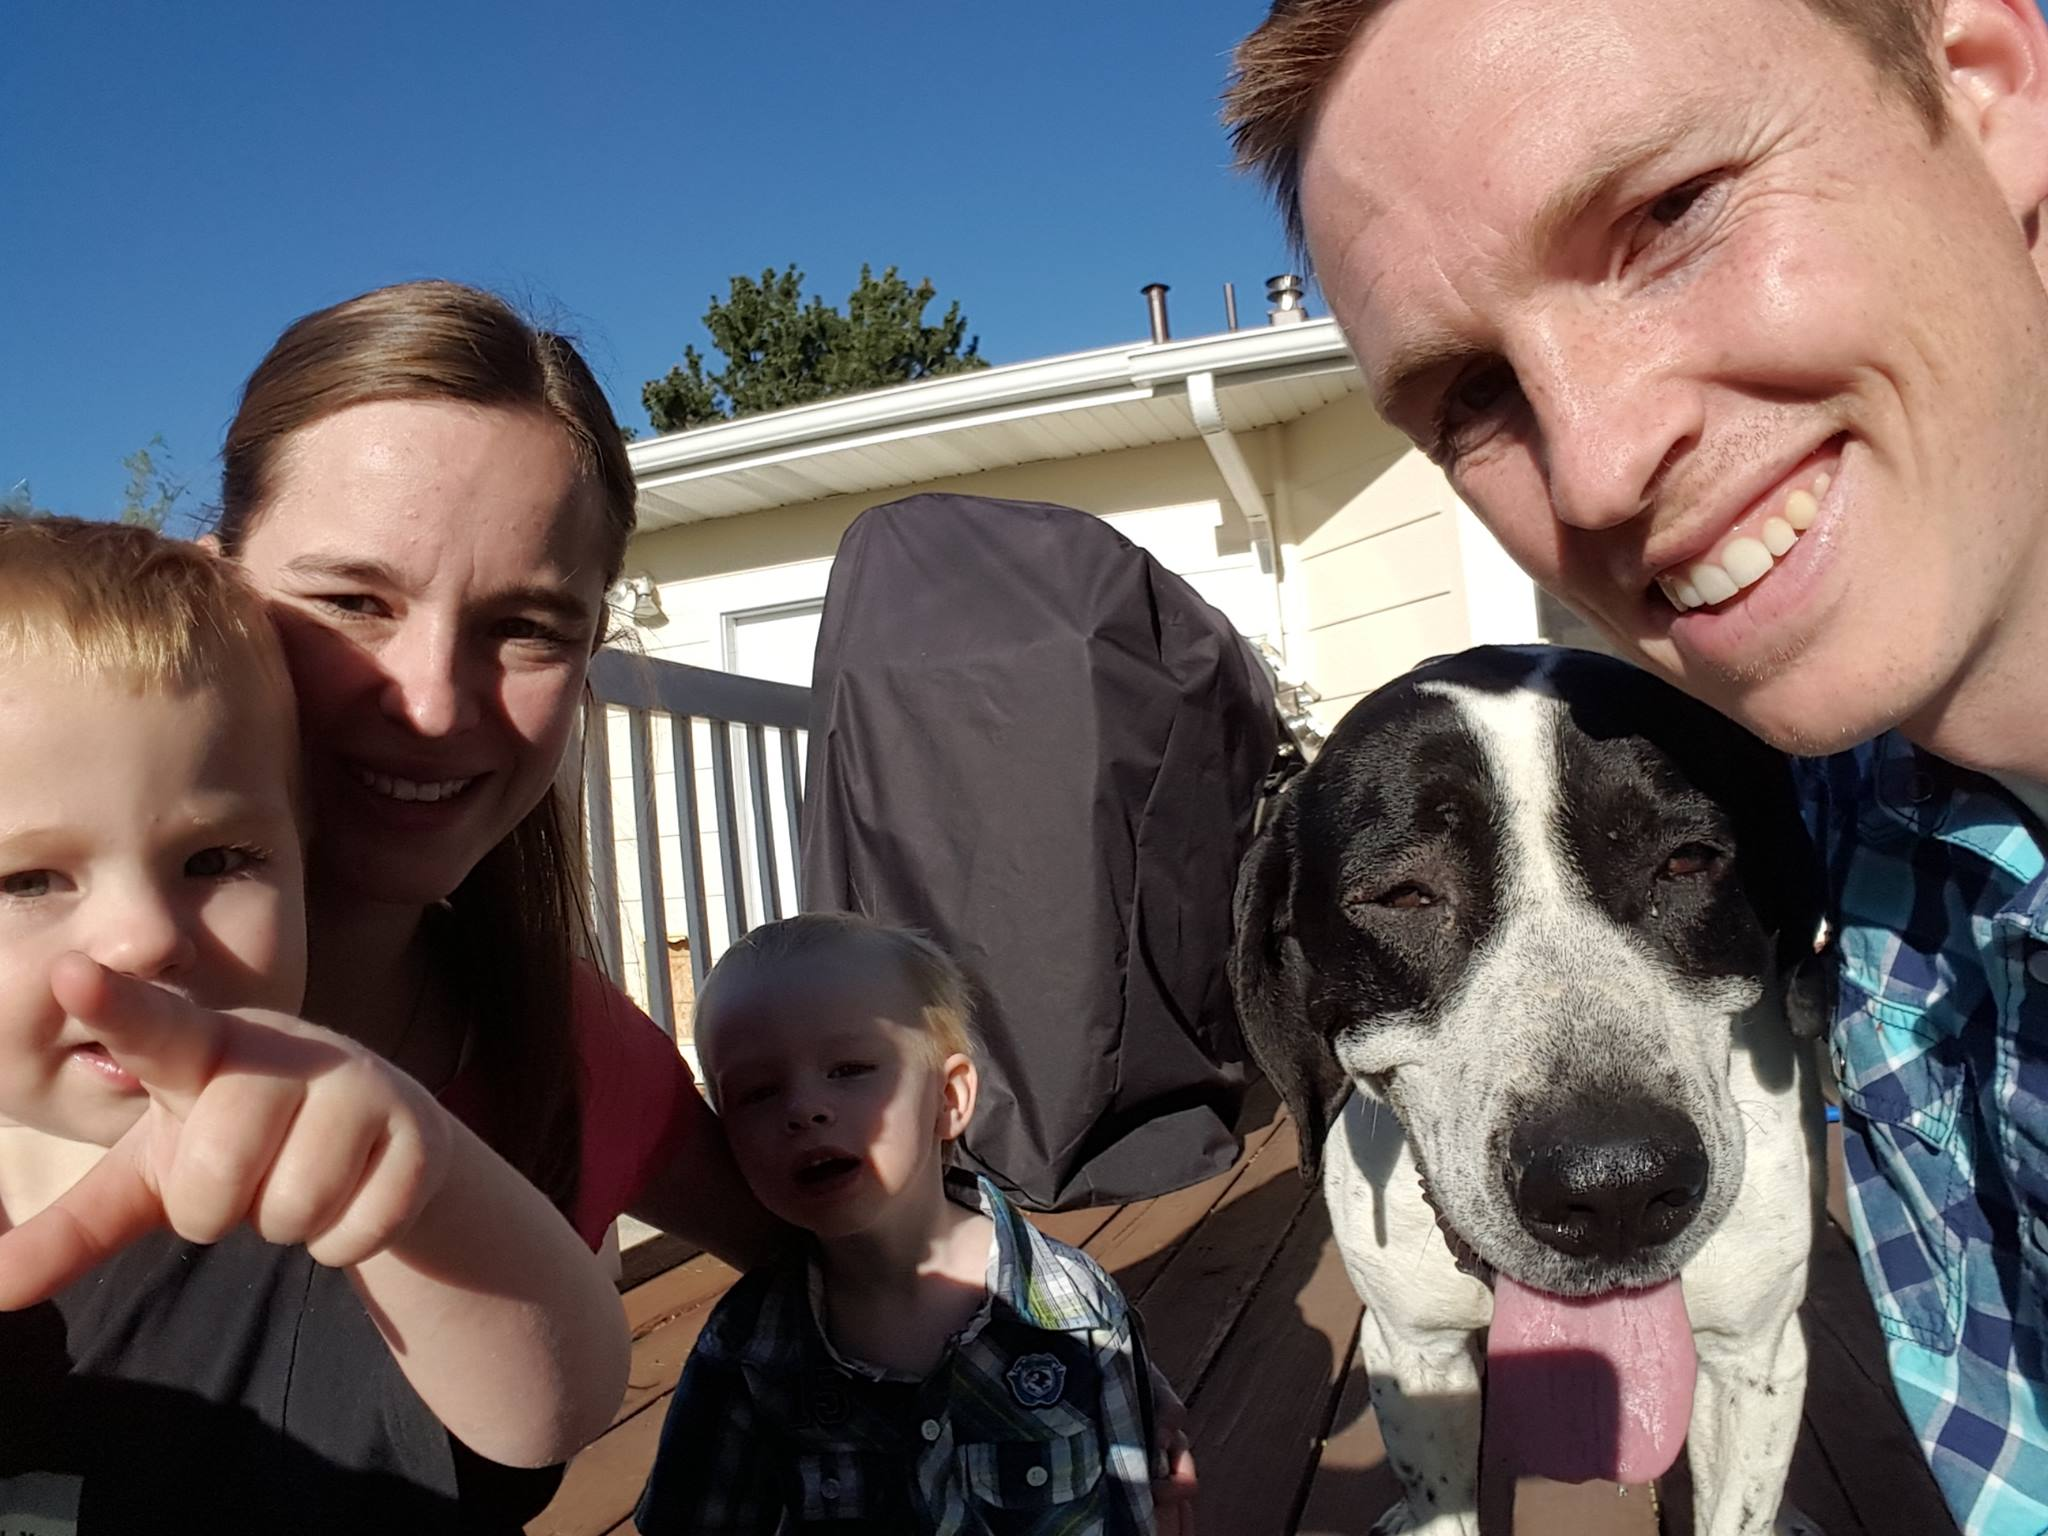
\includegraphics[width=3.8cm]{../figures/ziggy.jpg}
   \end{textblock*}
\end{frame}

\begin{frame}{Introduction}
\begin{center}
   \color{blue}{{\huge Two Truths and a Lie}}
\end{center}
\end{frame}
\fi

\begin{frame}{Motion Diagrams}
\begin{itemize}
   \item There are 4 types of motion that we are going to talk about. Can you name them (without looking at the book)?
\end{itemize}
\end{frame}

\begin{frame}{Motion Diagrams}
\begin{center}
   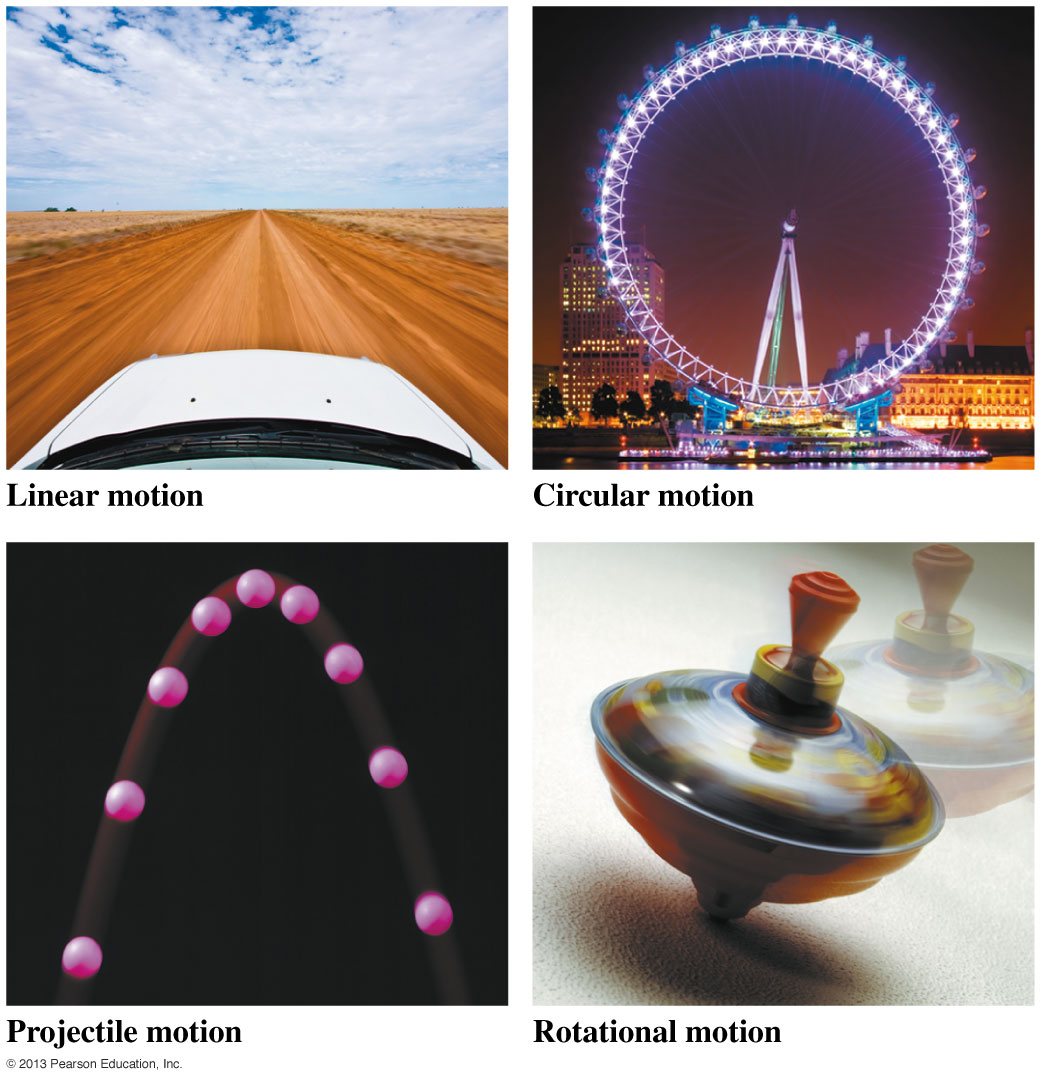
\includegraphics[height=0.9\textheight]{../figures/01_01_Figure.jpg}
\end{center}
\end{frame}

\begin{frame}{Motion Diagrams}
\begin{itemize}
   \item Before we start throwing around equations to talk about these types of motion lets figure out how to visualize physical situations in a useful way.
\end{itemize}
\end{frame}

\begin{frame}{Motion Diagrams}
\begin{itemize}
   \item<1-> On your whiteboards draw a picture describing the motion of the following situations
   \begin{itemize}[<+>]
      \item An rock sitting on the ground (just making sure you're awake)
      \item A car racing down the street but not changing speed
   \end{itemize}
   \only<3>{
   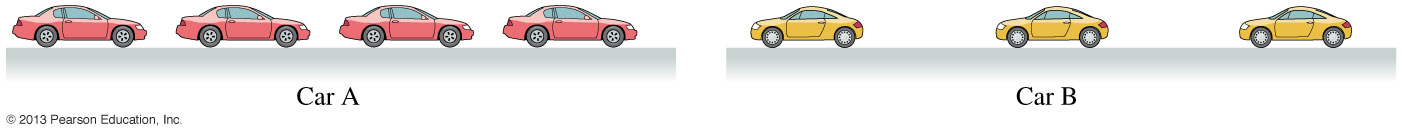
\includegraphics[width=0.9\textwidth]{../figures/Figure_STT1_1.jpg}
   \begin{center}
      Which car is going faster assuming time intervals are the same between frames?
   \end{center}
   }
   \pause
   \begin{itemize}[<+>]
      \item A football being thrown to a receiver
      \item A Semi truck hitting his breaks hard to stop at a red light
      \item Poe Dameron chasing down tie fighters in an X-wing
   \end{itemize}
   \item <7> This works as long as the pictures are simple, but what if they are really complicated?
\end{itemize}
\end{frame}

\begin{frame}{The Particle Model}
\begin{itemize}
   \item For many objects their general motion isn't determined by shape of the object so we can treat the object as if it had the same mass but all at one point.
   \begin{itemize}
      \item An object like this is called a \textbf{particle}.
   \end{itemize}
   \item This is called a model since it doesn't exactly represent reality: The \textbf{particle model}.
\end{itemize}
\end{frame}

\begin{frame}{The Particle Model}
\begin{center}
   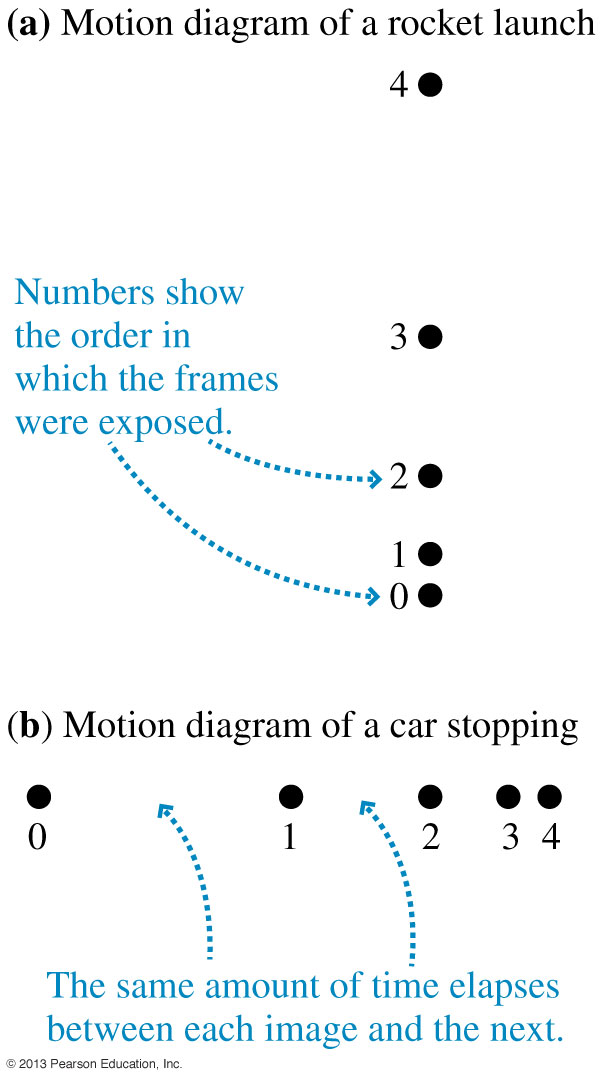
\includegraphics[height=0.9\textheight]{../figures/01_04_Figure.jpg}
\end{center}
\end{frame}

\begin{frame}{The Particle Model}
\begin{center}
   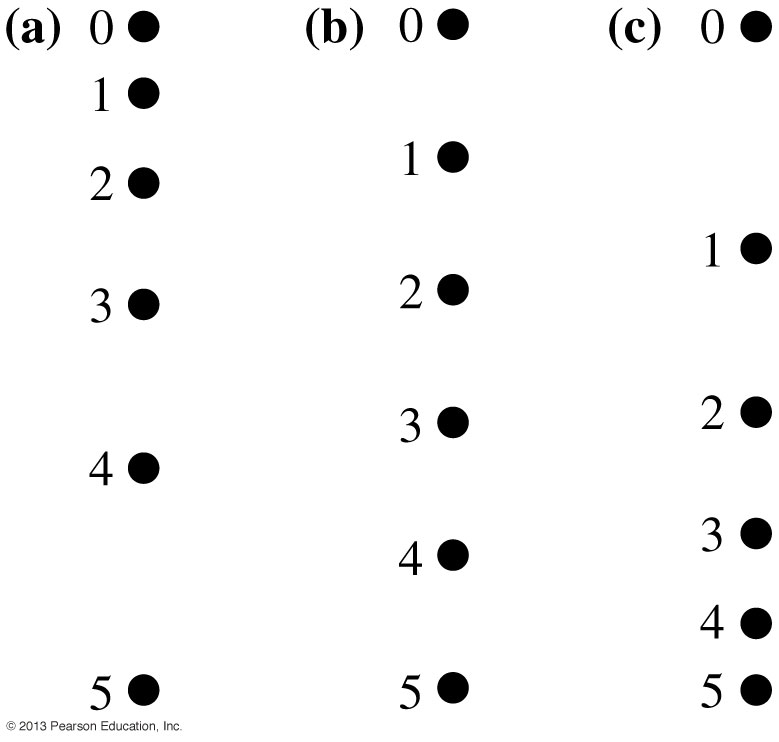
\includegraphics[width=0.5\textwidth]{../figures/Figure_STT1_2.jpg}
   \begin{enumerate}
      \item Dust particle settling ot the floor at constant speed.
      \item Ball dropped from the roof of a building.
      \item Descending rocket slowing to make a soft landing on Mars.
   \end{enumerate}
\end{center}
\end{frame}

\begin{frame}{The Particle Model}
\begin{itemize}
   \item Can you think of a situation for which the particle model doesn't do a good job describing the motion.
   \begin{itemize}
      \item<2> Rotating gear: the center of mass of the gear doesn't move but each individual tooth moves differently.
   \end{itemize}
\end{itemize}
\end{frame}

\begin{frame}{Position and Time}
\begin{center}
   \color{blue}{{\huge Position and Time}}
\end{center}
\end{frame}

\begin{frame}{Position and Time}
\begin{itemize}
   \item<1-> What is a coordinate system?
   \item<2-> Usually we think of x-y coordinate systems, but did you know that t could be a coordinate as well?
   \begin{center}
      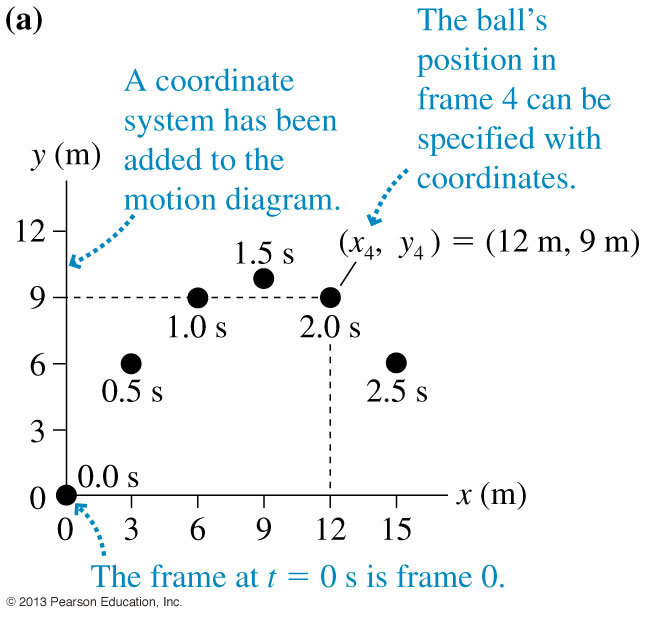
\includegraphics[width=0.5\textwidth]{../figures/01_05_FigureA.jpg}
   \end{center}
\end{itemize}
\end{frame}

\begin{frame}{Position and Time}
\begin{itemize}
   \item<1-> What is the origin of a coordinate system?
   \item<2-> What is the ``correct" origin for this room to describe the position of $<$insert item name$>$?
   \item<3-> What is the ``best" origin for this room to describe the position of $<$insert item name$>$?
\end{itemize}
\end{frame}

\begin{frame}{Position and Time}
\begin{itemize}
   \item<1-> What is a scalor? Give me some examples.
      \begin{itemize}
         \item<2-> Temperature, mass, age \ldots
      \end{itemize}
   \item<3-> What is a vector? Give me some examples.
      \begin{itemize}
         \item<4-> Velocity, position, forces \ldots \\~\\
         \begin{center}
            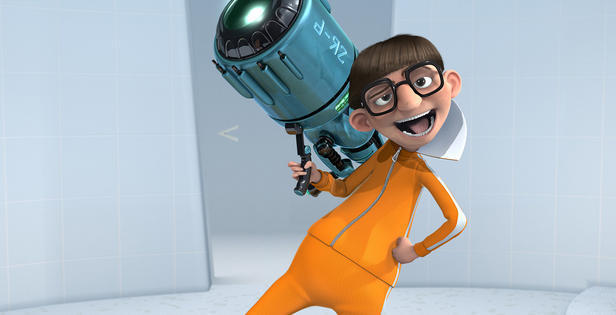
\includegraphics[width=0.5\textwidth]{../figures/Vector-_Despicable_Me.jpg}
         \end{center}
      \end{itemize}
      \item<5-> We give scalars symbols like $m$ and vectors symbols like $\vec{r}$.
      \item<6-> What is the difference between $r$ and $\vec{r}$ then?
\end{itemize}
\end{frame}

\begin{frame}{Position and Time}
\begin{itemize}
   \item Somebody come up and draw this situation labeling $\vec{r_0}$, $\vec{r_1}$ and $\Delta \vec{r}$.
   \item Sam is standing 50 ft east of the corner of 12th Street and Vine. He then walks northeast for 100 ft to the second point. What is Sam's change in position?
   \begin{itemize}
      \item This ($\Delta \vec{r}$) is called his \textbf{displacement}.
   \end{itemize}
\end{itemize}
\begin{center}
   \uncover<2>{
      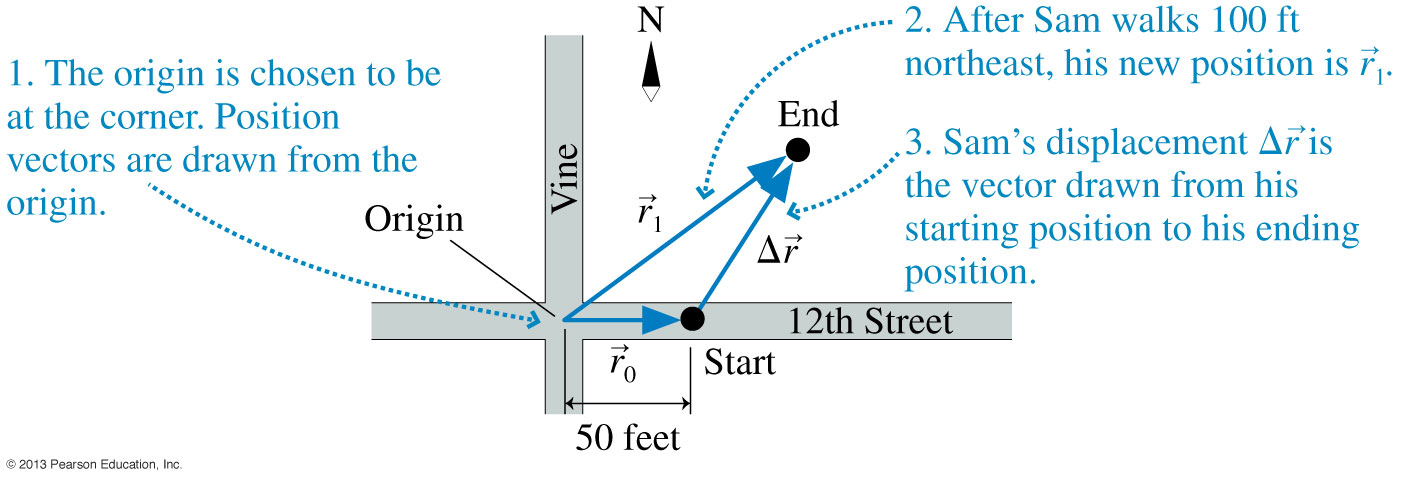
\includegraphics[width=0.8\textwidth]{../figures/01_06_Figure.jpg}
   }
\end{center}
\end{frame}

\begin{frame}{Position and Time}
\begin{itemize}
   \item You can write the displacement in different ways \ldots
   \begin{itemize}
      \item<1-> $\Delta \vec{r} = (100\mathrm{ft, northeast})$
      \item<2-> $\Delta \vec{r} = \vec{r}_f - \vec{r}_i$
   \end{itemize}
\end{itemize}
\begin{center}
   \uncover<2>{
      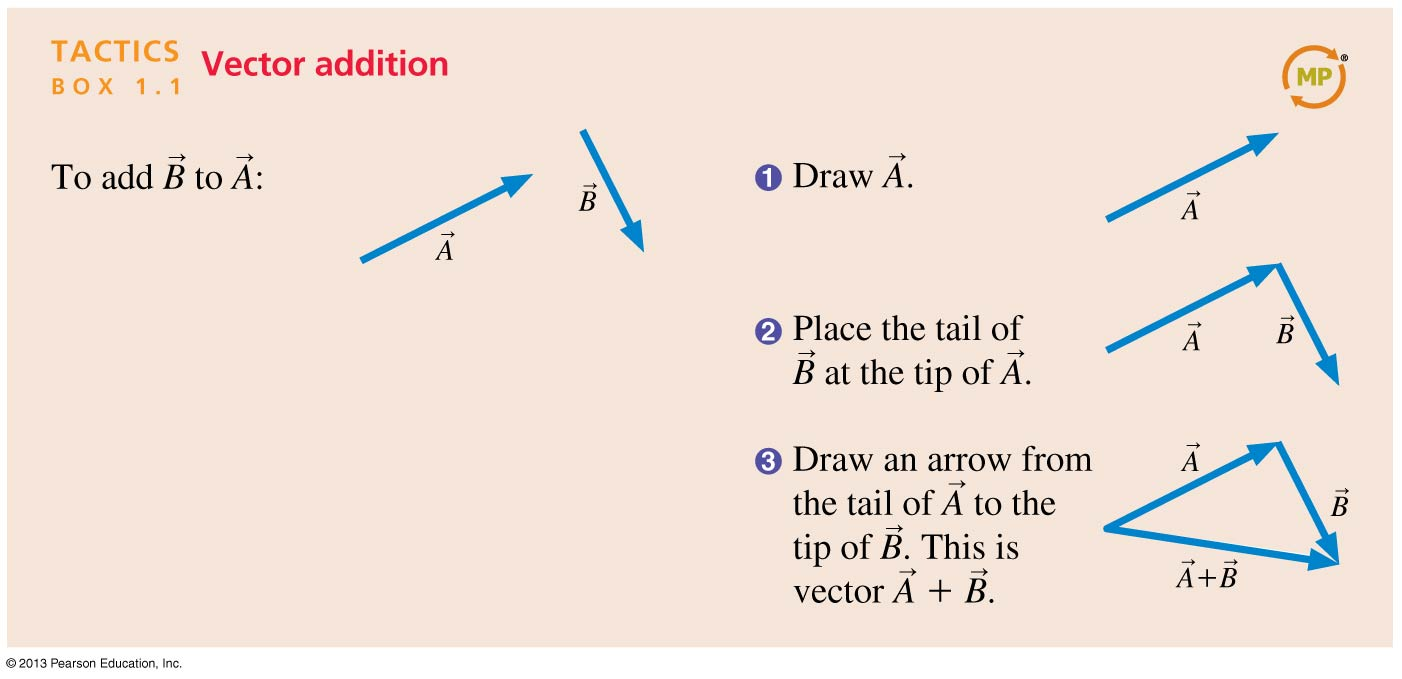
\includegraphics[width=0.8\textwidth]{../figures/tactics1_1.jpg}
   }
\end{center}
\end{frame}

\begin{frame}{Position and Time}
\begin{itemize}
   \item If that's how you add vectors, how would you subtract them?
\end{itemize}
\begin{center}
   \uncover<2>{
      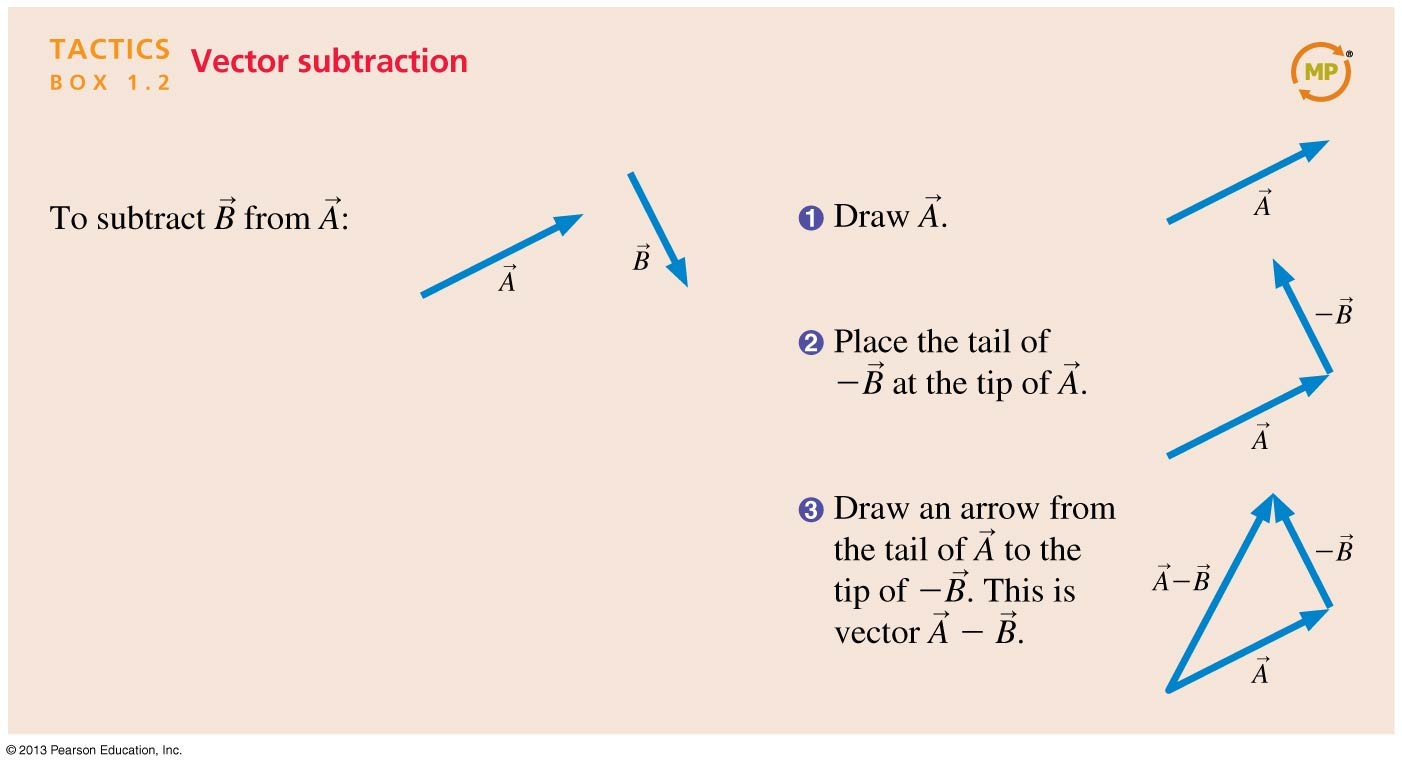
\includegraphics[width=0.8\textwidth]{../figures/tactics1_2.jpg}
   }
\end{center}
\end{frame}

\begin{frame}{Position and Time}
\begin{itemize}
   \item Why do we care about displacement?
   \begin{itemize}
      \item<2-> It's independent of coordinate system (and origin).
      \item<2-> Show this by moving the coordinate system to the right of the starting place and drawing vectors $\vec{r}_0$ and $\vec{r}_1$ again and subtract them to get $\Delta \vec{r} = \vec{r}_1 - \vec{r}_0$.
   \end{itemize}
\end{itemize}
\begin{center}
   \uncover<3>{
      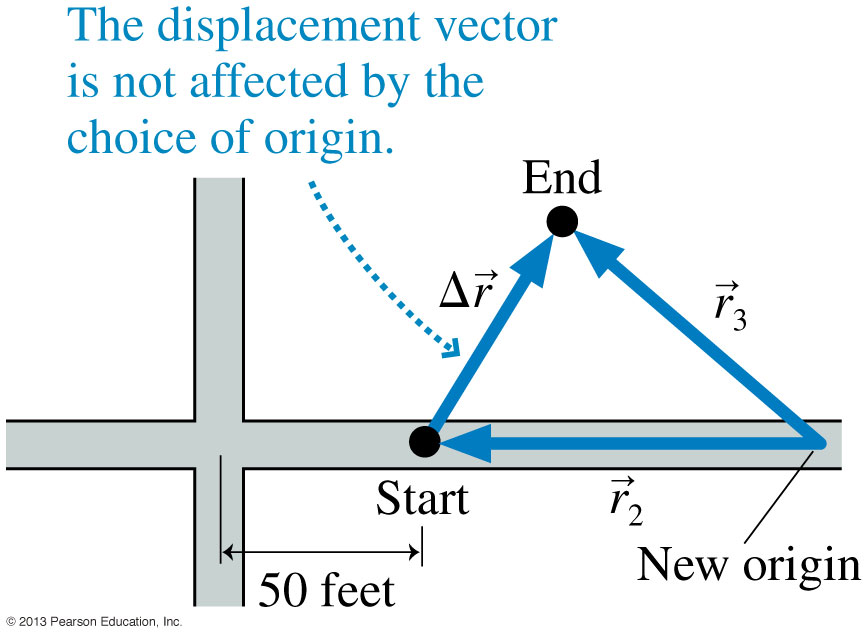
\includegraphics[width=0.5\textwidth]{../figures/01_07_Figure.jpg}
   }
\end{center}
\end{frame}

\begin{frame}{Position and Time}
\begin{itemize}
   \item Displacement vectors can be added to motion diagrams to give additional information.
\begin{columns}
   \begin{column}{0.4\textwidth}
   \begin{center}
      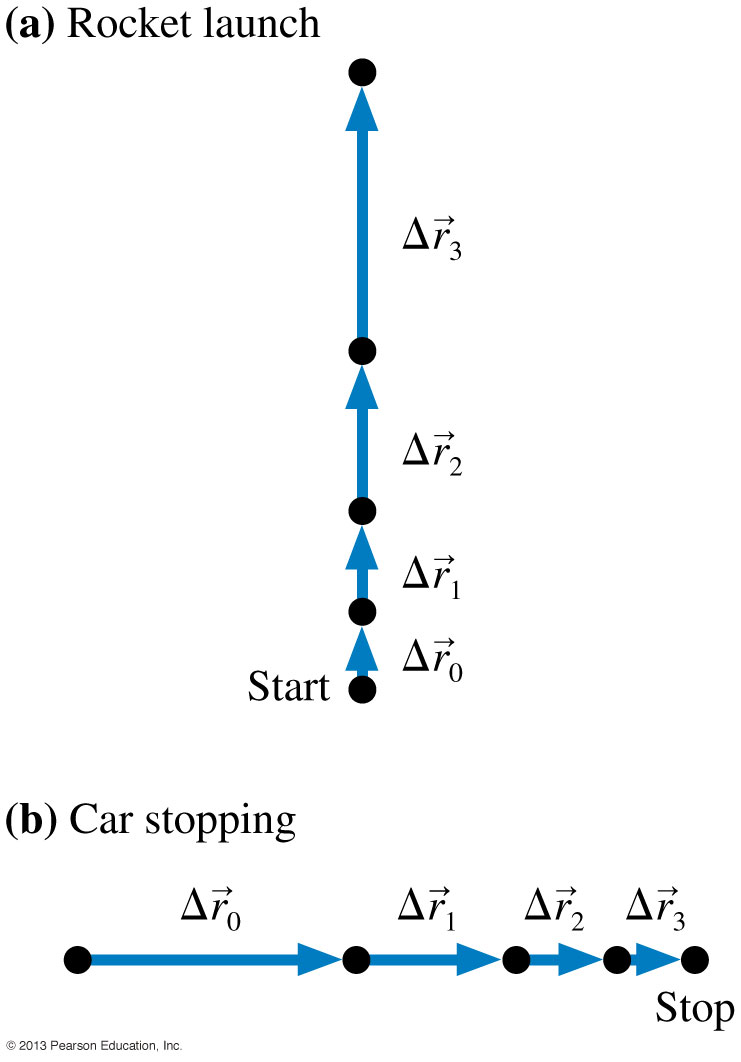
\includegraphics[width=\textwidth]{../figures/01_10_Figure.jpg}
   \end{center}
   \end{column}
   \begin{column}{0.6\textwidth}
      \begin{itemize}
         \item Speeding up: displacement vectors increase in length.
         \item Slowing down: displacement vectors decrease in length.
      \end{itemize}
   \end{column}
\end{columns}
\end{itemize}
\end{frame}

\begin{frame}{Position and Time}
\begin{itemize}
   \item The time interval, $\Delta t$, is like the displacement
   \begin{itemize}
      \item $\Delta t = t_f-t_i$
      \item Also, it doesn't depend on the origin ($t=0$)
   \end{itemize}
   \item People may disagree on the time that something happened, but they will always agree on the time interval between two events (At least in physics 121 dun dun duuuuun).
\end{itemize}
\end{frame}

\begin{frame}{Quick Check}
Which of these is $\vec{P}+\vec{Q}$?
\begin{center}
   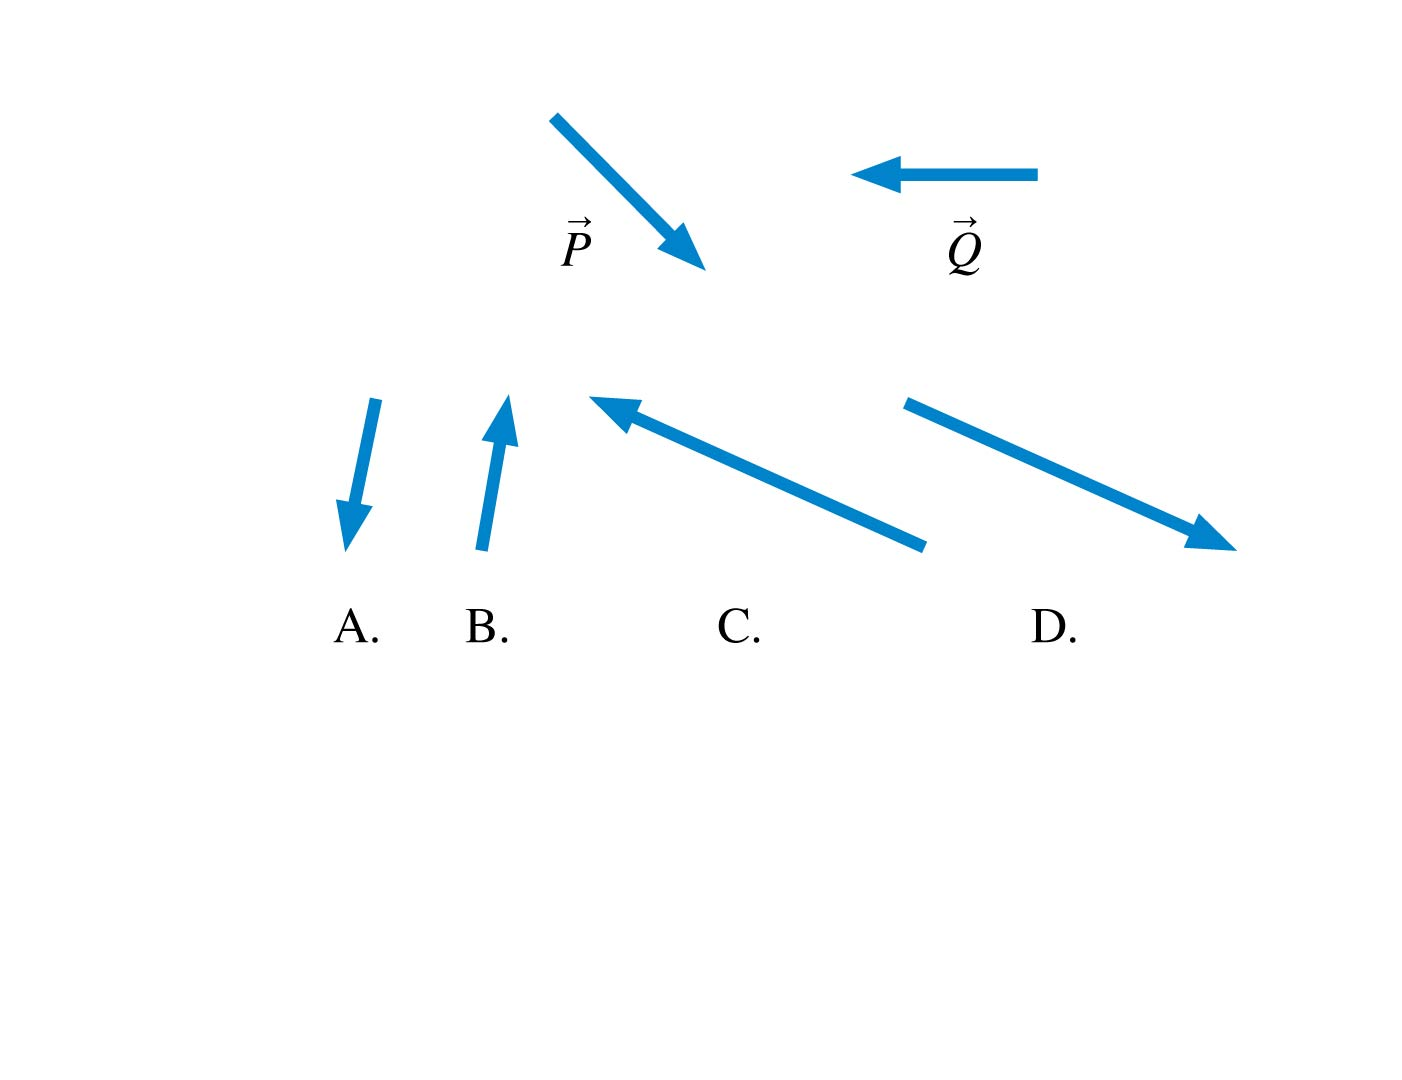
\includegraphics[width=1\textwidth]{../figures/QC1_3.jpg}
\end{center}
\only<2>{\checkH{3.3cm}{6.2cm}}
\end{frame}

\begin{frame}{Quick Check}
Which of these is $\vec{P}-\vec{Q}$?
\begin{center}
   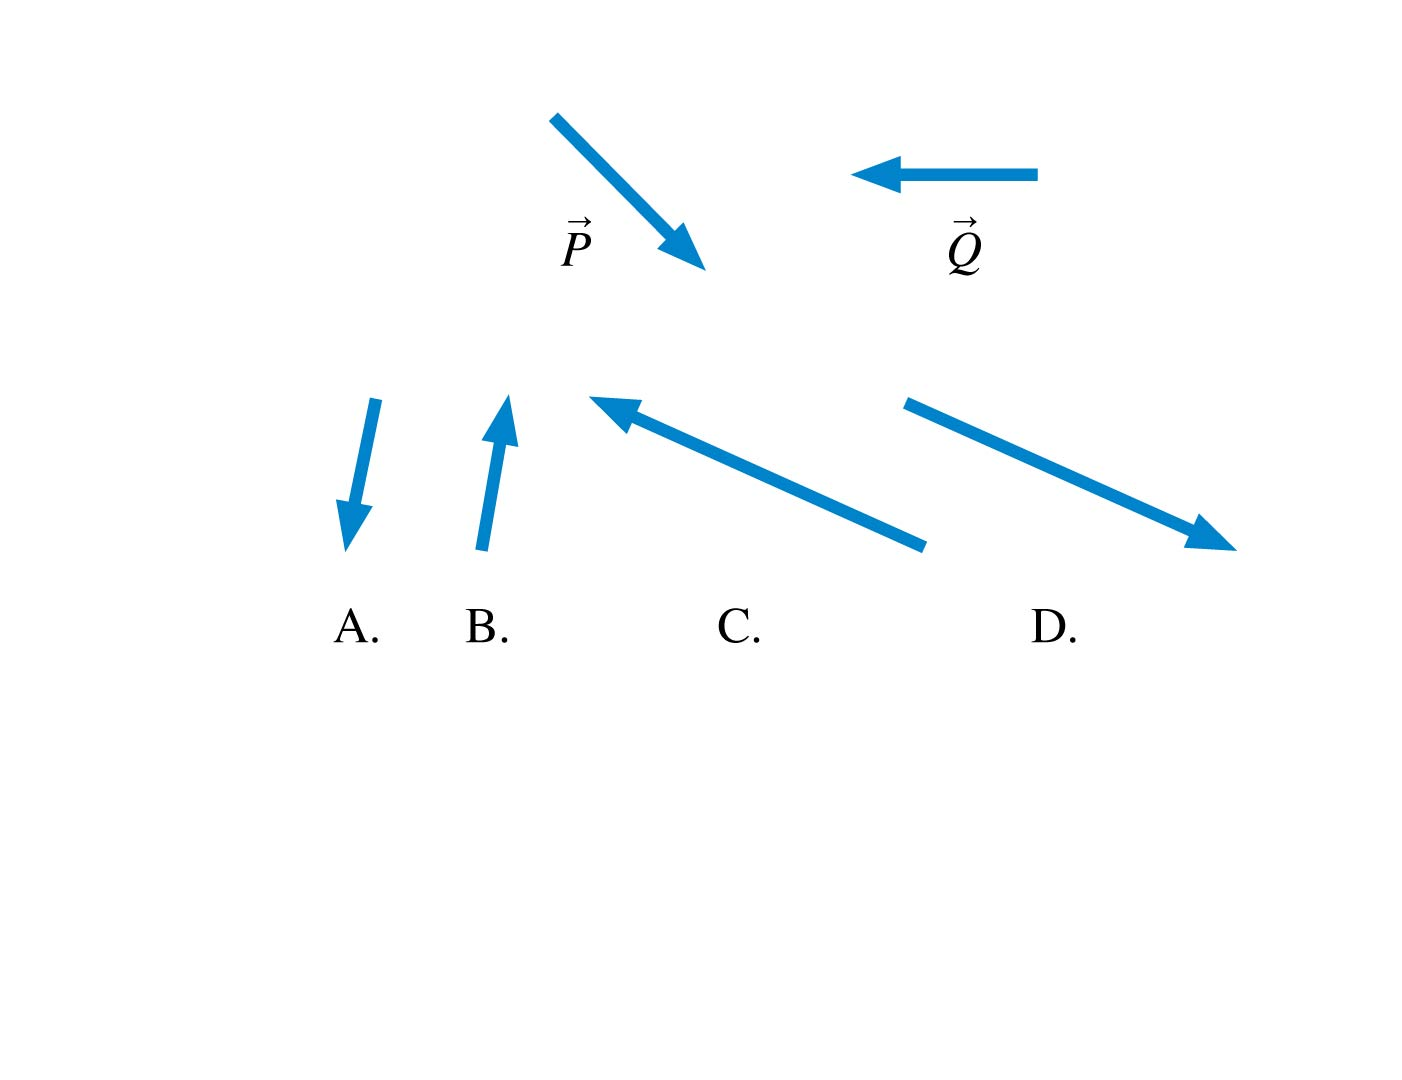
\includegraphics[width=1\textwidth]{../figures/QC1_3.jpg}
\end{center}
\only<2>{\checkH{9cm}{6.2cm}}
\end{frame}

\begin{frame}{REMINDER}
Just a reminder that we will have a quiz at the beginning of class on Thursday! It could be on what we have talked about or on the reading.
\end{frame}

\end{document}
